\chapter{\ifproject%
\ifenglish Project Structure and Methodology\else โครงสร้างและขั้นตอนการทำงาน\fi
\else%
\ifenglish Project Structure\else โครงสร้างของโครงงาน\fi
\fi
}

Overall, the methodologies involved data preprocessing, implementing 
two different recommendation algorithms \textit{(TF-IDF and KNN)}, 
combining their results into a hybrid approach, and integrating 
the system to become a part of backend system behind the e-Learning 
platform for user interaction and visualization of results. 
Here's a step-by-step summary of the experimentation and results:

\makeatletter

\section{Data Cleaning}
\begin{enumerate}
    \item \textsf{Load user and item datasets that are compatible with the specified format.}
    \item \textsf{In the user dataset, reformat dates, standardize payment statuses and education 
    levels, clean addresses, and extract email domains. Moreover, rename all columns}
    \item \textsf{In the item dataset, rename course and description columns}
    \item \textsf{After finishing all processes, save it to new files.}
\end{enumerate}

\begin{table}[htbp]
\center
\small
\begin{tabular}{p{1.1cm}p{1cm}p{0.5cm}p{2.5cm}p{1.75cm}p{1cm}p{1.75cm}p{1.7cm}} % Adjust column widths as needed
    \toprule
    \textbf{name} & \textbf{degree} & \textbf{Old}   & \textbf{your mail} & \textbf{residence}  & \textbf{course} & \textbf{enrollment} & \textbf{Is it paid} \\
    \midrule
    John       & 4-year     & 26           & john@gmail.com    & Bangkok & OOP  & yesterday     & success  \\
    Peter         & PHD        & 30     & peter@cmu.ac.th  &  &  Web & recent days    & failure \\
    thomas      & mid        & 42    & nelson@msn.com  & Chiang Mai & OS& a minute    & disapprove  \\
    \bottomrule
\end{tabular}
\caption{Before cleaning the user dataset}
\end{table}

\begin{table}[htbp]
\center
\small
\begin{tabular}{p{1.2cm}p{1.75cm}p{0.5cm}p{1.5cm}p{1.75cm}p{1.4cm}p{1.5cm}p{1.7cm}} % Adjust column widths as needed
    \toprule
    \textbf{username} & \textbf{education} & \textbf{age}   & \textbf{email} & \textbf{address}   & \textbf{course} & \textbf{time} & \textbf{payment} \\
    \midrule
    John          & Bachelor degree & 26           & gmail.com    & Bangkok  & OOP & 1/1/2566     & success  \\
    Peter         & Master degree & 30     & cmu.ac.th    &    & Web App & 1/5/2566  & failure \\
    thomas      & High school level & 42    & msn.com   & Chiang Mai & OS & 2/2/2566 & disapprove  \\
    \bottomrule
\end{tabular}
\caption{After cleaning the user dataset}
\end{table}

\begin{table}[H]
\center
\small
\begin{tabular}{p{3cm}p{10.85cm}}
    \toprule
    \textbf{Our Course Name} & \textbf{The Explanation} \\
    \midrule
    OOP &Object-Oriented Programming (OOP) allows for modular design, facilitating the organization 
    of recommendation system components into reusable and understandable classes. 
    Encapsulation ensures data integrity and abstraction simplifies complex algorithms, 
    enhancing maintainability and scalability. \\
    Web App &A web application is a software program accessed via web browsers over the internet. 
    It offers various services, from basic websites to complex systems. It uses a client-server 
    architecture for interaction, allowing modular design for scalability and flexibility. Technologies 
    like HTML, CSS, JavaScript, and server-side scripting languages enable development. \\
    OS &An operating system (OS) is software managing computer resources and providing a user interface. 
    It handles tasks such as process, memory, file, and device management, enabling multitasking and 
    efficient resource allocation. Encapsulation ensures data integrity, simplifies hardware interactions, 
    and enhances maintainability and scalability. Examples include Windows, macOS, Linux, and Unix. \\
    \bottomrule
\end{tabular}
\caption{Before cleaning the item dataset}
\end{table}

\begin{table}[H]
\center
\small
\begin{tabular}{p{3cm}p{10.85cm}}
    \toprule
    \textbf{Course} & \textbf{Description} \\
    \midrule
    OOP &Object-Oriented Programming (OOP) allows for modular design, facilitating the organization 
    of recommendation system components into reusable and understandable classes. 
    Encapsulation ensures data integrity and abstraction simplifies complex algorithms, 
    enhancing maintainability and scalability. \\
    Web App &A web application is a software program accessed via web browsers over the internet. 
    It offers various services, from basic websites to complex systems. It uses a client-server 
    architecture for interaction, allowing modular design for scalability and flexibility. Technologies 
    like HTML, CSS, JavaScript, and server-side scripting languages enable development. \\
    OS &An operating system (OS) is software managing computer resources and providing a user interface. 
    It handles tasks such as process, memory, file, and device management, enabling multitasking and 
    efficient resource allocation. Encapsulation ensures data integrity, simplifies hardware interactions, 
    and enhances maintainability and scalability. Examples include Windows, macOS, Linux, and Unix. \\
    \bottomrule
\end{tabular}
\caption{After cleaning the item dataset}
\end{table}

\newpage
\section{Course Recommendation using TF-IDF and Linear Kernel}
\begin{enumerate}
    \item \textsf{Load the cleaned dataset.}
    \item \textsf{Match courses between user dataset and item dataset to return descriptions.}
    \item \textsf{Use TF-IDF vectorization calculate the weights of words in the course descriptions.}
    \item \textsf{Apply linear kernel to calculate the cosine similarities between all courses.}
    \item \textsf{Return the top N recommended courses for the given courses taken by a specific user.}
\end{enumerate}

\subsection{Term Frequency}

\begin{equation}
    logNormalization(\text{term, document}) = 1 + log(f(term, document))
\end{equation}

\noindent Let's take an example of a course with the following description:
\begin{itemize}
    \item \texttt{\textbf{Doc}: The programming language is difficult, The local language is easy.}
\end{itemize}


\begin{itemize}
    \item[] \textbf{logTF}("The, Doc) \hspace{2cm} -> \hspace{0.5cm} 1 + log(2) $\approx$ 1.3
    \item[] \textbf{logTF}("programming, Doc) \hspace{0.43cm} -> \hspace{0.5cm} 1 + log(1) = 1
    \item[] \textbf{logTF}("language, Doc) \hspace{1.18cm} -> \hspace{0.5cm} 1 + log(2) $\approx$ 1.3
    \item[] \textbf{logTF}("is, Doc) \hspace{2.36cm} -> \hspace{0.5cm} 1 + log(2) $\approx$ 1.3
    \item[] \textbf{logTF}("difficult, Doc) \hspace{1.38cm} -> \hspace{0.5cm} 1 + log(1) = 1
    \item[] \textbf{logTF}("local, Doc) \hspace{1.85cm} -> \hspace{0.5cm} 1 + log(1) = 1
    \item[] \textbf{logTF}("easy, Doc) \hspace{1.94cm} -> \hspace{0.5cm} 1 + log(1) = 1
\end{itemize}

\subsection{Inverse Document Frequency}

\begin{equation}
    idf(term, allDocuments) = log \left( \frac{N}{df(term)} \right)
\end{equation}

\noindent Let's take an example of 2 courses with the following description:
\begin{itemize}
    \item \texttt{\textbf{Doc1}: The web programming language is taught by a foreign professor.}
    \item \texttt{\textbf{Doc2}: The network security is taught by a thai professor.}
\end{itemize}

\begin{itemize}
    \item[] \textbf{idf}("The", Doc1) \hspace{1.5cm} -> \hspace{0.5cm} log(2/2) = 0
    \item[] \textbf{idf}("web", Doc1) \hspace{1.47cm} -> \hspace{0.5cm} log(2/1) $\approx$ 0.3
    \item[] \textbf{idf}("network", Doc2) \hspace{0.83cm} -> \hspace{0.5cm} log(2/1) $\approx$ 0.3
    \item[] \textbf{idf}("professor", Doc2) \hspace{0.65cm} -> \hspace{0.5cm} log(2/2) = 0
\end{itemize}

\subsection{Term Frequency and Inverse Document Frequency}

\begin{equation}
    tfidf(term, document, allDocuments) = tf(term, document) \times idf(term, allDocuments)
\end{equation}

\noindent Let's take an example of a word 'language' that appears in 2 documents out of 3 documents.

\begin{itemize}
    \item \texttt{\textbf{Doc1}: The programming language is difficult, The local language is easy.}
    \item \texttt{\textbf{Doc2}: The web programming language is taught by a foreign professor.}
    \item \texttt{\textbf{Doc3}: The network security is taught by a thai professor.}
\end{itemize}

\begin{enumerate}
    \item \textbf{tf}("language", Doc1) = 1 + log(2) $\approx$ 1.3
    \item \textbf{idf}("language", [Doc1, Doc2, Doc3]) = log(3/2) $\approx$ 0.18
    \item \textbf{tfidf}("language", Doc1, [Doc1, Doc2, Doc3]) = 1.3 $\times$ 0.18 $\approx$ 0.23
\end{enumerate}

\subsection{Cosine Similarity}

\begin{equation}
    cosine\_similarity(A, B) = \frac{{A \cdot B}}{{\|A\| \cdot \|B\|}}
\end{equation}

\noindent Let's take an example of 3 courses with the following matrix 
where each row represents a course and each column represents a word:

\begin{table}[H]
\center
\begin{tabular}{|c|c|c|c|c|c|c|c|c|c|c|c|c|c|c|c|}
    \hline
        & \textbf{0} & \textbf{1} & \textbf{2} & \textbf{3} & \textbf{4} & \textbf{5} & \textbf{6} & \textbf{7} & \textbf{8} & \textbf{9} & \textbf{10} & \textbf{11} & \textbf{12} & \textbf{13} & \textbf{14} \\
    \hline
    \textbf{0} & 0.0 & 0.3 & 0.2 & 0.0 & 0.4 & 0.5 & 0.0 & 0.0 & 0.0 & 0.3 & 0.0 & 0.0 & 0.0 & 0.4 & 0.0 \\
    \hline
    \textbf{1} & 0.3 & 0.0 & 0.0 & 0.4 & 0.2 & 0.3 & 0.0 & 0.0 & 0.3 & 0.3 & 0.0 & 0.3 & 0.0 & 0.2 & 0.4 \\
    \hline
    \textbf{2} & 0.3 & 0.0 & 0.0 & 0.0 & 0.2 & 0.3 & 0.4 & 0.4 & 0.3 & 0.0 & 0.4 & 0.3 & 0.4 & 0.2 & 0.0 \\
    \hline
    \end{tabular}
\caption{User-Item Matrix}
\end{table}

\noindent Compute the \textit{dot product} between each pair of course vectors, 
so we get a course-course similarity matrix.

\begin{table}[H]
\[
\begin{bmatrix}
1 & 0.4493628 & 0.20315676 \\
0.4493628 & 1 & 0.44147846 \\
0.20315676 & 0.44147846 & 1 \\
\end{bmatrix}
\]
\caption{Item-Item Matrix}
\end{table}

\noindent We can finally use the this matrix to recommend courses based on a given course.

\section{Course Recommendation using Feature Ratings and KNN}
\begin{enumerate}
    \item \textsf{Load the cleaned dataset.}
    \item \textsf{Determine and calculate the feature ratings for each 
    course given by users.}
    \item \textsf{Train the model on the user-course to learn the relationships 
    between courses based on user preferences.}
    \item \textsf{Predict and rank the distances of courses based on the courses 
    that the user has taken.}
    \item \textsf{Return the top N recommended courses for the given user.}
\end{enumerate}

\subsection{Feature Ratings Calculation}

The \textit{feature ratings} are also considered to recommend courses to individual users.
The principle underlying this approach is to calculate the rating scores for each course 
based on the user's historical background. The measurement of impressive score is calculated 
by observing the behaviors of users in each column as follows.

\begin{itemize}
    \item \texttt{\textbf{Email} Column}
    \begin{itemize}
        \item[--] \texttt{Give 0 points if no email is provided.}
        \item[--] \texttt{Give 1 point if a common email domain is provided.}
        \item[--] \texttt{Give 2 points if an educational email domain is provided.}
    \end{itemize}
    \item \texttt{\textbf{Age-Education} Column}
    \begin{itemize}
        \item[--] \texttt{Give 0 points if a person is in the educational system.}
        \item[--] \texttt{Give 1 point if a person just graduated.}
        \item[--] \texttt{Give 2 points if a person is in the working age.}
    \end{itemize}
    \item \texttt{\textbf{Time} Column}
    \begin{itemize}
        \item[--] \texttt{Give 0 points if the time registration is unsuitable for a learning period.}
        \item[--] \texttt{Give 1 point if the time registration is suitable for a learning period.}
    \end{itemize}
    \item \texttt{\textbf{Payment} Column}
    \begin{itemize}
        \item[--] \texttt{Give 0 points if the payment is overdue.}
        \item[--] \texttt{Give 1 point if the payment is unapproved.}
        \item[--] \texttt{Give 2 points if the payment is on time.}
    \end{itemize}
    \item \texttt{\textbf{Address} Column}
    \begin{itemize}
        \item[--] \texttt{Give 0 points if the address is blank.}
        \item[--] \texttt{Give 1 point if the address is filled.}
    \end{itemize}
\end{itemize}

\noindent Find the \textit{impressive level} individually by considering the historical background of the user and the course.

\begin{table}[H]
\center
\begin{tabular}{|c|c|c|c|c|c|c|c|}
\hline
\textbf{User} &\textbf{Course} &\textbf{Email} &\textbf{Age-Education} &\textbf{Time} &\textbf{Payment} &\textbf{Address} &\textbf{Score} \\
\hline
User 1 & Course 1 & 0 & 0 & 1 & 1 & 1 & 2.75 \\
\hline
User 2 & Course 1 & 1 & 1 & 1 & 2 & 0 & 3.75 \\
\hline
User 3 & Course 3 & 2 & 0 & 0 & 0 & 0 & 1.75 \\
\hline
User 4 & Course 3 & 0 & 1 & 0 & 2 & 1 & 3.5 \\
\hline
User 5 & Course 2 & 1 & 2 & 0 & 0 & 0 & 1.875 \\
\hline
\end{tabular}
\caption{Feature Ratings}
\end{table}

\noindent Remove the feature rating columns to remain only user, course, and score.

\begin{table}[H]
\center
\begin{tabular}{|c|c|c|c|c|c|c|c|}
\hline
\textbf{User} & \textbf{Course} & \textbf{Score} \\
\hline
User 1 & Course 1 & 2.75 \\
\hline
User 2 & Course 1 & 3.75 \\
\hline
User 3 & Course 3 & 1.75 \\
\hline
User 4 & Course 3 & 3.5 \\
\hline
User 5 & Course 2 & 1.875 \\
\hline
\end{tabular}
\caption{Cleaned Feature Ratings}
\end{table}

\noindent Pivot the table to get the user-course matrix.

\begin{table}[H]
\center
\begin{tabular}{|c|c|c|c|c|c|}
\hline
& \textbf{User 1} & \textbf{User 2} & \textbf{User 3} & \textbf{User 4} & \textbf{User 5} \\
\hline
\textbf{Course 1} & 2.75 & 3.75 & NaN & NaN & NaN \\
\hline
\textbf{Course 2} & NaN & NaN & NaN & NaN & 1.875 \\
\hline
\textbf{Course 3} & NaN & NaN & 1.75 & 3.5 & NaN \\
\hline
\end{tabular}
\caption{User-Course Matrix}
\end{table}

\newpage
\subsection{Nearest Neighbors Model}

\noindent Fit a k-nearest neighbors (KNN) model. Where 
yellow, red, and blue colours represent 3 different courses.

% \vspace{10pt}
\begin{figure}[H]
\center
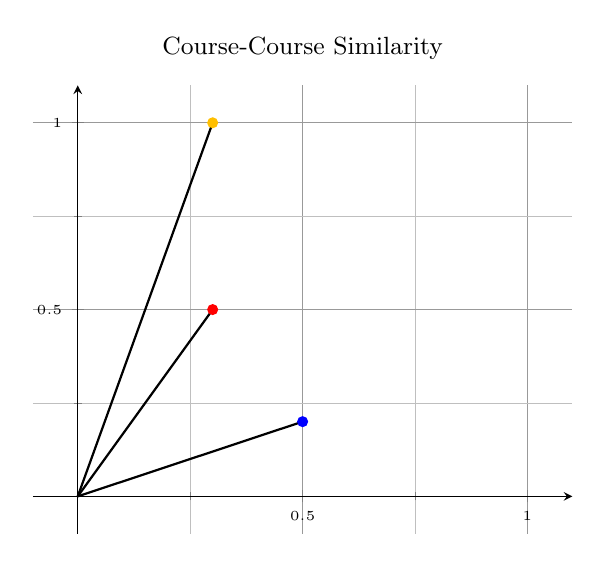
\begin{tikzpicture}
\begin{axis}[
    xmin=0, xmax=1,
    ymin=0, ymax=1,
    xtick={0,0.5,1},
    ytick={0,0.5,1},
    grid=both,
    grid style={line width=0.2pt, draw=gray!50},
    major grid style={line width=0.4pt,draw=gray!80},
    minor tick num=1,
    axis line style={-},
    axis lines=middle,
    enlargelimits=true,
    ticklabel style={font=\tiny},
    label style={font=\small},
    title={Course-Course Similarity},
    title style={font=\small,align=center},
    nodes near coords={
        \pgfmathprintnumber{\pgfplotspointmeta}
    },
    every node near coord/.append style={
        anchor=west,
        font=\footnotesize,
        yshift=2pt, % adjust vertical position of the label
        xshift=-5pt % adjust horizontal position of the label
    }
]
\addplot[
    scatter,
    only marks,
    mark=*,
    mark size=2pt,
    scatter src=explicit,
    scatter/use mapped color={draw opacity=0,fill=mapped color}
]
table[x=x, y=y, meta=meta] {
    x y meta
    0.5 0.2 1
    0.3 1 2
    0.3 0.5 3
};

\draw[thick,-] (axis cs:0.5,0.2) -- (axis cs:0,0);
\draw[thick,-] (axis cs:0.3,1) -- (axis cs:0,0);
\draw[thick,-] (axis cs:0.3,0.5) -- (axis cs:0,0);

\end{axis}
\end{tikzpicture}
\caption{KNN Model}
\end{figure}

\noindent Use the KNN model to calculate the cosine distance between the red course and all other courses. 

\begin{table}[H]
\center
\begin{tabular}{|c|c|}
\hline
\textbf{Course} & \textbf{Cosine Distance} \\
\hline
yellow & 0.25 \\
blue & 0.4 \\
\hline
\end{tabular}
\caption{Predicted Distances}
\end{table}

\noindent After calculating the cosine distances for all courses, select the top most similar courses.

\section{Hybrid Course Recommendation}
\begin{enumerate}
    \item \textsf{Loaded the cleaned dataset.}
    \item \textsf{Combined the results from TF-IDF and KNN approaches using 
    a hybrid recommendation system.}
    \item \textsf{Returned the top N recommended courses for the given user, 
    integrating recommendations from both TF-IDF and KNN approaches.}
\end{enumerate}

\vspace{25pt}
\subsection{The combination of TF-IDF and KNN}

Set the weights and normalize the matrices of TF-IDF and KNN.
\begin{table}[H]
    \centering
    \vspace{10pt}
    \begin{tabular}{|c|c|c|c|c|c|}
        \hline
        & \textbf{User 1} & \textbf{User 2} & \textbf{User 3} & \textbf{User 4} & \textbf{User 5} \\
        \hline
        \textbf{Course 1} & 1.00 & 3.75 & 2.00 & 2.50 & 3.25 \\
        \hline
        \textbf{Course 2} & 2.25 & 2.75 & 1.75 & 1.50 & 1.87 \\
        \hline
        \textbf{Course 3} & 1.00 & 1.40 & 1.95 & 4.55 & 4.45 \\
        \hline
    \end{tabular}
    \caption{Before the normalization}
    \vspace{10pt}
    \begin{tabular}{|c|c|c|c|c|c|}
        \hline
        & \textbf{User 1} & \textbf{User 2} & \textbf{User 3} & \textbf{User 4} & \textbf{User 5} \\
        \hline
        \textbf{Course 1} & 0.167 & 0.626 & 0.334 & 0.417 & 0.543 \\
        \hline
        \textbf{Course 2} & 0.486 & 0.594 & 0.378 & 0.324 & 0.404 \\
        \hline
        \textbf{Course 3} & 0.145 & 0.204 & 0.284 & 0.662 & 0.647 \\
        \hline
    \end{tabular}
    \caption{After the normalization}
\end{table}

\noindent Stack arrays in sequence horizontally

\begin{table}[htbp]
    \centering
    \begin{minipage}[t]{0.4\textwidth} % Adjust the width as needed
        \centering
        \begin{tabular}{|c|c|c|}
        \hline
        & Column 1 & Column 2 \\
        \hline
        Row 1 & 0.1 & 0.2  \\
        Row 2 & 0.3 & 0.4 \\
        Row 3 & 0.5 & 0.6 \\
        \hline
        \end{tabular}
        \caption{Matrix 1}
    \end{minipage}
    \hspace{20pt} % Adjust the horizontal space between tables
    \begin{minipage}[t]{0.4\textwidth} % Adjust the width as needed
        \centering
        \begin{tabular}{|c|c|}
        \hline
        & Column 3\\
        \hline
        Row 1 & 0.7 \\
        Row 2 & 0.8 \\
        Row 3 & 0.9 \\
        \hline
        \end{tabular}
        \caption{Matrix 2}
    \end{minipage}
\end{table}

\begin{table}[htbp]
    \centering
    \begin{tabular}{|c|c|c|c|}
    \hline
    & Column 1 & Column 2 & Column 3 \\
    \hline
    Row 1 & 0.1 & 0.2 & 0.7 \\
    Row 2 & 0.3 & 0.4 & 0.8 \\
    Row 3 & 0.5 & 0.6 & 0.9 \\
    \hline
    \end{tabular}
    \caption{Stacked Matrix}
\end{table}

\subsection{The process of Recommendation}

We apply Nearest Neighbors to the stacked matrix to get the final recommendation.
Nevertheless, the process of recommendation is the same as the KNN approach.

\newpage

\section{Evaluation}

By following this evaluation process, developers and researchers can measure and improve the 
effectiveness of recommendation systems in providing personalized and relevant recommendations to users.

\begin{enumerate}
    \item \textsf{Consider users who have taken more than one course.}
    \item \textsf{The training and testing datasets are splitted by identifying the ratio.}
    \item \textsf{Allow the model to familiarize itself with the training dataset to ensure there is no bias.}
    \item \textsf{Predict the courses for all users using the trained model.}
    \item \textsf{Calculate the accuracy by measuring the similarities between the predicted courses and the actual test courses.}
    \item \textsf{Investigate the results and adjust the parameters to enhance the quality of the system.}
\end{enumerate}

\subsection{Training and Testing}

In designing the training and testing split, several considerations can be made to ensure an effective 
evaluation of the recommendation system. These considerations include:

\begin{enumerate}
    \item \textsf{\textbf{Consider only users who have taken more than 1 course: }
    This step ensures that you have enough data from each user for meaningful analysis.}
    \item \textsf{\textbf{Divide the courses into 2 parts individually according to the specified proportions: }
    This ensures that each user's data is divided according to the specified proportion.}
    \item \textsf{\textbf{Split the dataset corresponding to the curriculum from step 2: }
        This ensures that the dataset is approximately divided into two parts: one for training and one for testing.}
\end{enumerate}

\subsection{Accuracy Measurement}
There are two performance measurements in total including \textit{hit rate} and \textit{f1 score}.

\subsubsection{Hit Rate}

A Hit measures the share of users that get at least one relevant recommendation. Hit Rate is calculated as follows:

\begin{equation}
    \text{HitRate} = \frac{\texttt{Number of Hits}}{\texttt{Number of Users}}
\end{equation}

\noindent A larger value of recommended courses can potentially improve the hit rate because it provides more opportunities to include relevant items. Therefore, the performance of the hit rate indeed depends on the number of recommended courses.


\subsubsection{F1 Score}

Recall, Precision, and F1 Score can use the following formulas:

\begin{equation}
    Recall = \frac{\texttt{Number of correctly predicted items}}{\texttt{Total number of relevant items}}
\end{equation}

\begin{equation}
    Precision = \frac{\texttt{Number of correctly predicted items}}{\texttt{Total number of recommended items}}
\end{equation}

\begin{equation}
    F1\_score = \frac{2⋅Precision⋅Recall}{Precision+Recall}
\end{equation}

\begin{itemize}
    \item \texttt{Number of correctly predicted items - The course that system predict correctly.}
    \item \texttt{Total number of relevant items - The courses that have been taken by the user from the course recommendation system}
    \item \texttt{Total number of recommended items - All courses that the recommendation system suggests for user}
\end{itemize}

\noindent To find the average F1 score from all users by

\begin{equation}
    \text{$F1\_score_{average}$} = \frac{\sum_{i=1}^{n}F1\_score_{i}}{\texttt{Number of Users}}
\end{equation}

\noindent The harmonic mean nature makes sure if either Precision or Recall has a really high value, then it does not dominate the score. F1 Score has a high value when both precision and recall values are close to 1.

\newpage
\section{Function Structure}

\subsection{The TfidfLinearKernel class}

\subsubsection{\textcolor{red}{The fit(item\_df) method}}

\vspace{-7mm}
\begin{table}[H]
\small
\begin{tabularx}{\textwidth}{|p{2cm}|X|}
\hline
\textbf{Parameters} & \textbf{item\_df:} \textit{pd.DataFrame} \\ & \hspace{5mm} The DataFrame that contains course and description columns. \\
\textbf{Returns} & \textbf{matrix:} \textit{sparse matrix of (n\_sample, n\_features)} \\ & \hspace{5mm} The TF-IDF-Weighted document-term matrix. \\
\hline
\end{tabularx}
\end{table}

\subsubsection{\textcolor{red}{The predict(name, item\_df, user\_df, matrix, n\_recommendations=10) method}}

\vspace{-7mm}
\begin{table}[H]
\small
\begin{tabularx}{\textwidth}{|p{2cm}|X|}
\hline
\textbf{Parameters} & \textbf{name:} \textit{str} \\ & \hspace{5mm} A name of user \\
& \textbf{item\_df:} \textit{pd.DataFrame} \\ & \hspace{5mm} The DataFrame that contains course and description columns. \\
& \textbf{user\_df:} \textit{pd.DataFrame} \\ & \hspace{5mm} The DataFrame that contains user, course, and features columns. \\
& \textbf{matrix:} \textit{sparse matrix of (n\_sample, n\_features)} \\ & \hspace{5mm} The TF-IDF-Weighted document-term matrix. \\
& \textbf{n\_recommendations:} \textit{int, default=10} \\ & \hspace{5mm} The number of recommended courses. \\
\textbf{Returns} & \textbf{prediction\_df:} \textit{pd.DataFrame} \\ & \hspace{5mm} The DataFrame that contains recommended course with score columns \\
\hline
\end{tabularx}
\end{table}

\subsubsection{\textcolor{red}{The train\_test\_split(user\_df, test\_size=0.2) method}}

\vspace{-7mm}
\begin{table}[H]
\small
\begin{tabularx}{\textwidth}{|p{2cm}|X|}
\hline
\textbf{Parameters} & \textbf{user\_df:} \textit{pd.DataFrame} \\ & \hspace{5mm} The DataFrame that contains user, course, and features columns. \\
& \textbf{test\_size:} \textit{float, default=0.2} \\ & \hspace{5mm} The proportion of the DataFrame to include in the test split. \\
\textbf{Returns} & \textbf{X\_train:} \textit{pd.DataFrame} \\ & \hspace{5mm} The training DataFrame. \\
& \textbf{X\_test:} \textit{pd.DataFrame} \\ & \hspace{5mm} The testing DataFrame. \\
\hline
\end{tabularx}
\end{table}

\subsubsection{\textcolor{red}{The hit\_rate(train, test, item\_data, matrix, k=10) method}}

\vspace{-7mm}
\begin{table}[H]
\small
\begin{tabularx}{\textwidth}{|p{2cm}|X|}
\hline
\textbf{Parameters} & \textbf{train:} \textit{pd.DataFrame} \\ & \hspace{5mm} The training DataFrame. \\
& \textbf{test:} \textit{pd.DataFrame} \\ & \hspace{5mm} The testing DataFrame. \\
& \textbf{item\_df:} \textit{pd.DataFrame} \\ & \hspace{5mm} The DataFrame that contains course and description columns. \\
& \textbf{matrix:} \textit{sparse matrix of (n\_sample, n\_features)} \\ & \hspace{5mm} The TF-IDF-Weighted document-term matrix. \\
& \textbf{k:} \textit{int, default=10} \\ & \hspace{5mm} The number of recommendations to consider. \\
\textbf{Returns} & \textbf{hit\_rate:} \textit{float} \\ & \hspace{5mm} The hit rate of the recommendation system. \\
\hline
\end{tabularx}
\end{table}

\subsubsection{\textcolor{red}{The f1\_score(train, test, item\_data, model, k=10) method}}

\vspace{-7mm}
\begin{table}[H]
\small
\begin{tabularx}{\textwidth}{|p{2cm}|X|}
\hline
\textbf{Parameters} & \textbf{train:} \textit{pd.DataFrame} \\ & \hspace{5mm} The training DataFrame. \\
& \textbf{test:} \textit{pd.DataFrame} \\ & \hspace{5mm} The testing DataFrame. \\
& \textbf{item\_df:} \textit{pd.DataFrame} \\ & \hspace{5mm} The DataFrame that contains course and description columns. \\
& \textbf{matrix:} \textit{sparse matrix of (n\_sample, n\_features)} \\ & \hspace{5mm} The TF-IDF-Weighted document-term matrix. \\
& \textbf{k:} \textit{int, default=10} \\ & \hspace{5mm} The number of recommendations to consider. \\
\textbf{Returns} & \textbf{f1\_score:} \textit{float} \\ & \hspace{5mm} The F1 score of the recommendation system. \\
\hline
\end{tabularx}
\end{table}

\subsection{The FeatureRatingsKNN Class}

\subsubsection{\textcolor{red}{The fit(user\_data) method}}

\vspace{-7mm}
\begin{table}[H]
\small
\begin{tabularx}{\textwidth}{|p{2cm}|X|}
\hline
\textbf{Parameters} & \textbf{user\_data:} \textit{pd.DataFrame} \\ & \hspace{5mm} The DataFrame that contains user-item data. \\
\textbf{Returns} & \textbf{model:} \textit{NearestNeighbors} \\ & \hspace{5mm} The fitted nearest neighbors estimator. \\
\hline
\end{tabularx}
\end{table}

\subsubsection{\textcolor{red}{The predict(name, user\_data, model, n\_recommendations=10) method}}

\vspace{-7mm}
\begin{table}[H]
\small
\begin{tabularx}{\textwidth}{|p{2cm}|X|}
\hline
\textbf{Parameters} & \textbf{name:} \textit{str} \\ & \hspace{5mm} The name of the user. \\
& \textbf{user\_data:} \textit{pd.DataFrame} \\ & \hspace{5mm} The DataFrame that contains user-item data. \\
& \textbf{model:} \textit{NearestNeighbors} \\ & \hspace{5mm} The fitted nearest neighbors estimator. \\
& \textbf{n\_recommendation:} \textit{int, default=10} \\ & \hspace{5mm} The number of top items to recommend. \\
\textbf{Returns} & \textbf{prediction\_df:} \textit{pd.DataFrame} \\ & \hspace{5mm} The DataFrame that contains recommended course with score columns \\
\hline
\end{tabularx}
\end{table}

\subsubsection{\textcolor{red}{The train\_test\_split(user\_data, test\_size=0.2) method}}

\vspace{-7mm}
\begin{table}[H]
\small
\begin{tabularx}{\textwidth}{|p{2cm}|X|}
\hline
\textbf{Parameters} & \textbf{user\_data:} \textit{pd.DataFrame} \\ & \hspace{5mm} The DataFrame that contains user-item data. \\
& \textbf{test\_size:} \textit{float, default=0.2} \\ & \hspace{5mm} The proportion of the DataFrame to include in the test split. \\
\textbf{Returns} & \textbf{train:} \textit{pd.DataFrame} \\ & \hspace{5mm} The training DataFrame. \\
& \textbf{test:} \textit{pd.DataFrame} \\ & \hspace{5mm} The testing DataFrame. \\
\hline
\end{tabularx}
\end{table}

\subsubsection{\textcolor{red}{The hit\_rate(train, test, model, k=10) method}}

\vspace{-7mm}
\begin{table}[H]
\small
\begin{tabularx}{\textwidth}{|p{2cm}|X|}
\hline
\textbf{Parameters} & \textbf{train:} \textit{pd.DataFrame} \\ & \hspace{5mm} The training DataFrame. \\
& \textbf{test:} \textit{pd.DataFrame} \\ & \hspace{5mm} The testing DataFrame. \\
& \textbf{model:} \textit{NearestNeighbors} \\ & \hspace{5mm} The fitted nearest neighbors estimator. \\
& \textbf{k:} \textit{int, default=10} \\ & \hspace{5mm} The number of recommendations to consider. \\
\textbf{Returns} & \textbf{hit\_rate:} \textit{float} \\ & \hspace{5mm} The hit rate of the recommendation system. \\
\hline
\end{tabularx}
\end{table}

\subsubsection{\textcolor{red}{The f1\_score(train, test, model, k=10) method}}

\vspace{-7mm}
\begin{table}[H]
\small
\begin{tabularx}{\textwidth}{|p{2cm}|X|}
\hline
\textbf{Parameters} & \textbf{train:} \textit{pd.DataFrame} \\ & \hspace{5mm} The training DataFrame. \\
& \textbf{test:} \textit{pd.DataFrame} \\ & \hspace{5mm} The testing DataFrame. \\
& \textbf{model:} \textit{NearestNeighbors} \\ & \hspace{5mm} The fitted nearest neighbors estimator. \\
& \textbf{k:} \textit{int, default=10} \\ & \hspace{5mm} The number of recommendations to consider. \\
\textbf{Returns} & \textbf{f1\_score:} \textit{float} \\ & \hspace{5mm} The F1 score of the recommendation system. \\
\hline
\end{tabularx}
\end{table}

\subsection{The Hybrid Class}

\subsubsection{\textcolor{red}{The fit(item\_data, user\_data) method}}

\vspace{-7mm}
\begin{table}[H]
\small
\begin{tabularx}{\textwidth}{|p{2cm}|X|}
\hline
\textbf{Parameters} & \textbf{item\_df:} \textit{pd.DataFrame} \\ & \hspace{5mm} The DataFrame that contains course and description columns. \\
& \textbf{user\_data:} \textit{pd.DataFrame} \\ & \hspace{5mm} The DataFrame that contains user-item data. \\
\textbf{Returns} & \textbf{model:} \textit{NearestNeighbors} \\ & \hspace{5mm} The fitted nearest neighbors estimator. \\
\hline
\end{tabularx}
\end{table}

\subsubsection{\textcolor{red}{The predict(name, item\_data, user\_data, model, n\_recommendations=10) method}}

\vspace{-7mm}
\begin{table}[H]
\small
\begin{tabularx}{\textwidth}{|p{2cm}|X|}
\hline
\textbf{Parameters} & \textbf{name:} \textit{str} \\ & \hspace{5mm} A name of user \\
& \textbf{item\_df:} \textit{pd.DataFrame} \\ & \hspace{5mm} The DataFrame that contains course and description columns. \\
& \textbf{user\_data:} \textit{pd.DataFrame} \\ & \hspace{5mm} The DataFrame that contains user-item data. \\
& \textbf{model:} \textit{NearestNeighbors} \\ & \hspace{5mm} The fitted nearest neighbors estimator. \\
& \textbf{n\_recommendations:} \textit{int, default=10} \\ & \hspace{5mm} The number of recommended courses. \\
\textbf{Returns} & \textbf{prediction\_df:} \textit{pd.DataFrame} \\ & \hspace{5mm} The DataFrame that contains recommended course with score columns \\
\hline
\end{tabularx}
\end{table}

\subsubsection{\textcolor{red}{The train\_test\_split(item\_data, test\_size=0.2) method}}

\vspace{-7mm}
\begin{table}[H]
\small
\begin{tabularx}{\textwidth}{|p{2cm}|X|}
\hline
\textbf{Parameters} & \textbf{item\_df:} \textit{pd.DataFrame} \\ & \hspace{5mm} The DataFrame that contains course and description columns. \\
& \textbf{test\_size:} \textit{float, default=0.2} \\ & \hspace{5mm} The proportion of the DataFrame to include in the test split. \\
\textbf{Returns} & \textbf{train:} \textit{pd.DataFrame} \\ & \hspace{5mm} The training DataFrame. \\
& \textbf{test:} \textit{pd.DataFrame} \\ & \hspace{5mm} The testing DataFrame. \\
\hline
\end{tabularx}
\end{table}

\subsubsection{\textcolor{red}{The hit\_rate(train, test, model, k=10) method}}

\vspace{-7mm}
\begin{table}[H]
\small
\begin{tabularx}{\textwidth}{|p{2cm}|X|}
\hline
\textbf{Parameters} & \textbf{train:} \textit{pd.DataFrame} \\ & \hspace{5mm} The training DataFrame. \\
& \textbf{test:} \textit{pd.DataFrame} \\ & \hspace{5mm} The testing DataFrame. \\
& \textbf{model:} \textit{NearestNeighbors} \\ & \hspace{5mm} The fitted nearest neighbors estimator. \\
& \textbf{k:} \textit{int, default=10} \\ & \hspace{5mm} The number of recommendations to consider. \\
\textbf{Returns} & \textbf{hit\_rate:} \textit{float} \\ & \hspace{5mm} The hit rate of the recommendation system. \\
\hline
\end{tabularx}
\end{table}

\subsubsection{\textcolor{red}{The f1\_score(train, test, model, k=10) method}}

\vspace{-7mm}
\begin{table}[H]
\small
\begin{tabularx}{\textwidth}{|p{2cm}|X|}
\hline
\textbf{Parameters} & \textbf{train:} \textit{pd.DataFrame} \\ & \hspace{5mm} The training DataFrame. \\
& \textbf{test:} \textit{pd.DataFrame} \\ & \hspace{5mm} The testing DataFrame. \\
& \textbf{model:} \textit{NearestNeighbors} \\ & \hspace{5mm} The fitted nearest neighbors estimator. \\
& \textbf{k:} \textit{int, default=10} \\ & \hspace{5mm} The number of recommendations to consider. \\
\textbf{Returns} & \textbf{f1\_score:} \textit{float} \\ & \hspace{5mm} The F1 score of the recommendation system. \\
\hline
\end{tabularx}
\end{table}
